\chapter{System Requirements}


\section{Requirements}
From discussions with a social entrepreneur, founder and CEO of Anudip Dr. Radha Basu, and by reflecting on our own experiences working abroad with social enterprises, we have compiled the following requirements for this project. Functional requirements are quantitative and describe the actual functions our system needs to be able to perform, while nonfunctional requirements are qualitative and describe the way in which the functional requirements are implemented. \\[-0.7\baselineskip]

\underline{Functional}\\
\textit{Critical}
\begin{itemize}
\item Trainers are able to make training materials available to trainees digitally.
\item Trainers are able to test trainees’ knowledge of training materials.
\item Trainers are able to view results of quizzes.
\item Trainers are able to enable/disable quizzes.
\item Trainers are able to register/unregister trainees for use of system.
\item Trainees are able to access training materials.
\item Trainees are able to receive training materials in small pieces.
\end{itemize}

\textit{Recommended}
\begin{itemize}
\item Trainers are able to send notifications when new training materials are added.
\item Trainees are able to automatically receive results from quiz.
\item Trainees are able to view their progress.
\item Trainees are able to access notifications/training materials multiple times.
\end{itemize}

\textit{Suggested}
\begin{itemize}
\item Trainers are able to set a time limit on the completion of quizzes.\\[-0.5\baselineskip]
\end{itemize}

\underline{Non-Functional}\\*
\textit{Critical}
\begin{itemize}
\item Compatible with basic/feature phones.
\item Easy to read.
\item Low distribution costs for social enterprises.
\item Portable to different web and mobile platforms.
\item Maintainable.
\end{itemize}

\textit{Recommended}
\begin{itemize}
\item Scalable for more users.
\end{itemize}

\textit{Suggested}
\begin{itemize}
\item Open source, extensible.
\item Support for multiple languages.
\end{itemize}

\section{Use Cases}
For our implementation, we have come up with several key use cases for the two types of users of our system: trainers and trainees. The following figures visually describe the main functions for each type of user. The primary use cases are also described in greater detail below.

\begin{figure}[H]
	\centering
	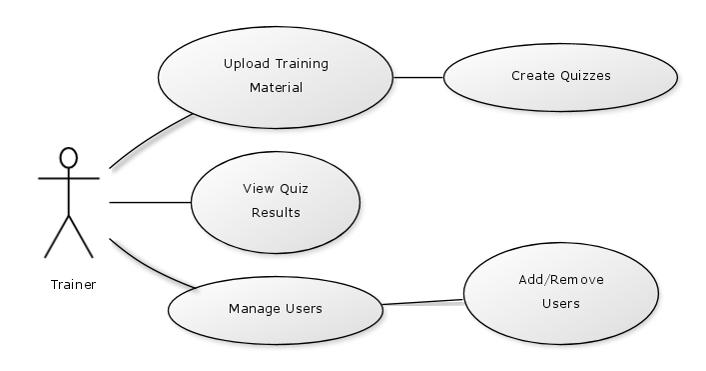
\includegraphics[scale=0.6]{use_case_trainer.png}
	\caption{Use Case for Trainers}
\end{figure}

\begin{figure}[H]
	\centering
	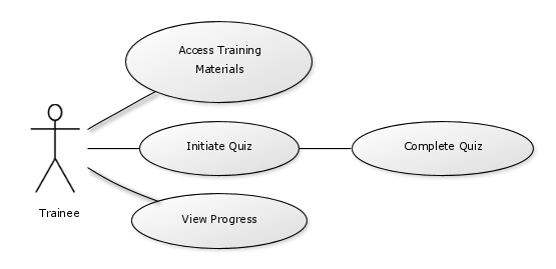
\includegraphics[scale=0.6]{use_case_trainee.png}
	\caption{Use Case for Trainees}
\end{figure}


\underline{Case 1 - Upload Training Material}\\*
\textit{Actor:} Trainer\\*
\textit{Goal:} Materials with related quiz are ready to distribute.\\*
\textit{Preconditions:} Have materials in a plaintext format, be a registered user, and internet connection.\\*
\textit{Postconditions:} Materials are uploaded and a quiz is created.\\*
\textit{Scenario:}
\begin{enumerate}
	\item{Navigate to the “Add New Materials” page.}
	\item{Enter text of training materials into the box.}
	\item{Write in the questions answers in the appropriate boxes.}
	\item{Hit Submit.}
\end{enumerate}
\textit{Exceptions:}
\begin{enumerate}
	\item{Text is too long to process.}
	\item{Something on the site is broken.}\\
\end{enumerate}

\underline{Case 2 - Add User}\\*
\textit{Actor:} Trainer\\*
\textit{Goal:} Grant access to training materials to their employees.\\*
\textit{Preconditions:} Be a registered user, know the phone-number the employee will be using.\\*
\textit{Postconditions:} A registered user can download training materials.\\*
\textit{Scenario:}
\begin{enumerate}
	\item{Navigate to the ``Manage Users'' page.}
	\item{Select “Add Contact” from the action list.}
	\item{Enter the new user’s name and mobile number.}
	\item{Hit ``Save'' to store the number and send a verification text to the trainee.}
\end{enumerate}
\textit{Exceptions:}
\begin{enumerate}
	\item{Incorrect mobile number.}\\
\end{enumerate}

\underline{Case 3 - Manage/Edit Training Materials}\\*
\textit{Actor:} Trainer\\*
\textit{Goal:} Ability to view and edit all uploaded training materials, quizzes, and related SMS messages.\\*
\textit{Preconditions:} Be a registered user, have previously uploaded training materials, and internet connection.\\*
\textit{Postconditions:} Training materials can be edited.\\*
\textit{Scenario:}
\begin{enumerate}
	\item{Navigate to the ``Training Materials'' page.}
	\item{To add a new training material, click on ``Add new'' within the Training Materials Panel.}
	\item{To view or edit an existing training material, click on ``List Training Materials'' in the action list and then click on the title of the desired training material.}
	\item{Once a training material has been saved, it can be previewed by clicking ``Preview'' at the bottom of its edit page.}
	\item{To assign and send a training material to users, select ``Assign'' next to the desired training material from the main ``List Training Materials'' page, check users to assign to, and click ``Assign and Send Notification''.}
\end{enumerate}
\textit{Exceptions:}
\begin{enumerate}
	\item{Cannot edit texts that have already been sent; must send new version.}\\
\end{enumerate}

\underline{Case 4 - Initiate and Take Quiz}\\*
\textit{Actor:} Trainee\\*
\textit{Goal:} Respond to quizzes based on specific training materials.\\*
\textit{Preconditions:} Trainee is registered by trainer and has received and completed reading training materials on phone.\\*
\textit{Postconditions:} Trainee can submit responses to quiz.\\*
\textit{Scenario:}
\begin{enumerate}
	\item{Receive assignment notification text message with instructions on how to begin quiz.}
	\item{Reply to message following the instructions to begin quiz.}
	\item{Receive quiz questions one at a time on phone as SMS messages.}
	\item{Answer questions by texting back answer along with appropriate tag.}
	\item{Receive feedback and correct answer if applicable.}
	\item{Quiz results are sent back to webpage to be parsed and stored in cloud.}
\end{enumerate}
\textit{Exceptions:}
\begin{enumerate}
	\item{Quiz is not available.}
\end{enumerate}